\documentclass[letterpaper,12pt]{article}

% things needed to include figures
\usepackage{subfigure, graphicx}
% float must be included for the [H] to actually work
\usepackage{float}
% formulas
\usepackage{amsmath}
% Added to adjust captions
\usepackage[singlelinecheck=false]{caption}
% added to adjust margins at the suggestion of Dr. Matt
\usepackage[top=1in, bottom=1in, left=1in, right=1in]{geometry}
\usepackage{fullpage}
\title{The Speed of Light}
\author{Max Bigras and David Frawley}

\begin{document}

\maketitle

\section{The speed of light}
\subsection{Light speed in air}
Using a pulse modulated diode laser and fast photodiode detector we measured the time lag between the laser pulse and detection. We adjusted the distance the laser pulse traveled in air using mirrors. By plotting distance vs. time, shown in Figure \ref{air}, we determined $c^{\mathrm{air}}_{\mathrm{exp}} = 3.02 \times 10^{8} \pm 0.03 $ m/s, which agrees with the accepted value, $c^{\mathrm{air}} = 2.99792458 \times 10^{8}$ m/s.
\begin{figure}[H]
  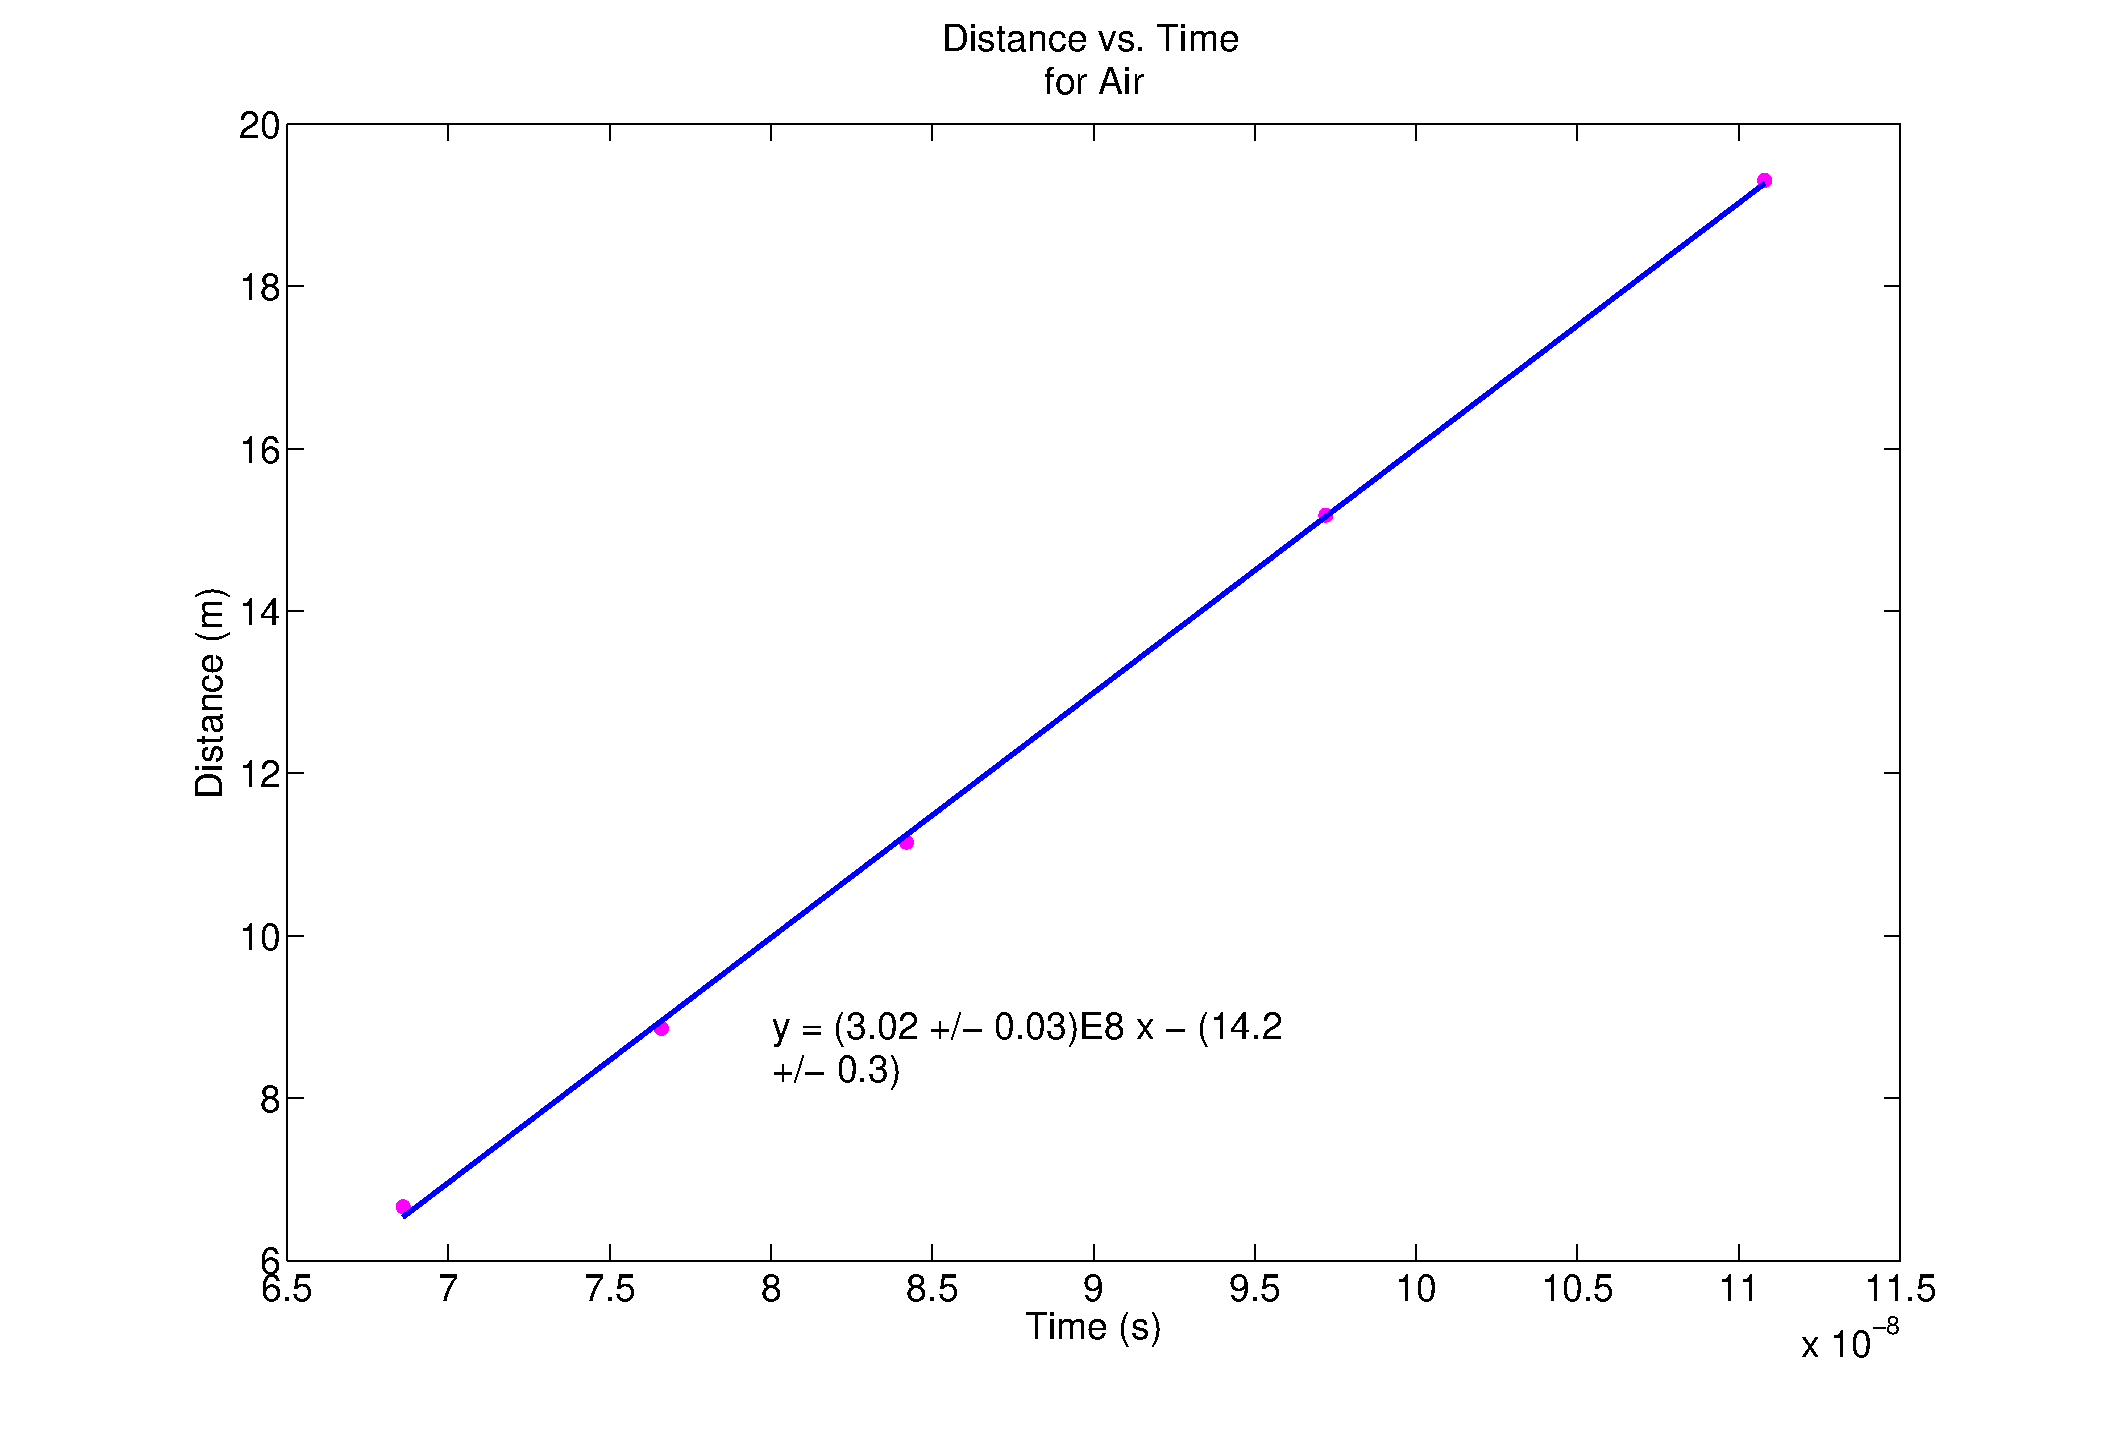
\includegraphics[totalheight=0.6\textwidth]{figs/air_final}
  \caption{Determining the speed of light in air}
  \label{air}
\end{figure}

\subsection{Light speed in an optical fiber}
Using a pulse modulated diode laser and fast photodiode detector we measured the time lag between the laser pulse and detection. We adjusted the distance the laser pulse traveled in an optical fiber by using different lengths of fiber. By plotting distance vs. time, shown in Figure \ref{fiber}, we determined $c^{\mathrm{fiber}}_{\mathrm{exp}} = 1.85 \times 10^{8} \pm 0.03 $ m/s. The refractive index for a material is given by the equation
\begin{equation}
n^{\mathrm{material}} = c^{\mathrm{vacuum}}/c^{\mathrm{material}}
\label{n}
\end{equation}

Applying Equation \ref{n} and using $c^{\mathrm{air}}_{\mathrm{exp}} \approx c^{\mathrm{vacuum}}$ we determined $n^{\mathrm{fiber}}_{\mathrm{exp}} = 1.63 \pm 0.01$ which agrees with the accepted value for the core of a optical fiber $n^{\mathrm{fiber}} \approx 1.62$ \cite{wiki}.

\begin{figure}[H]
  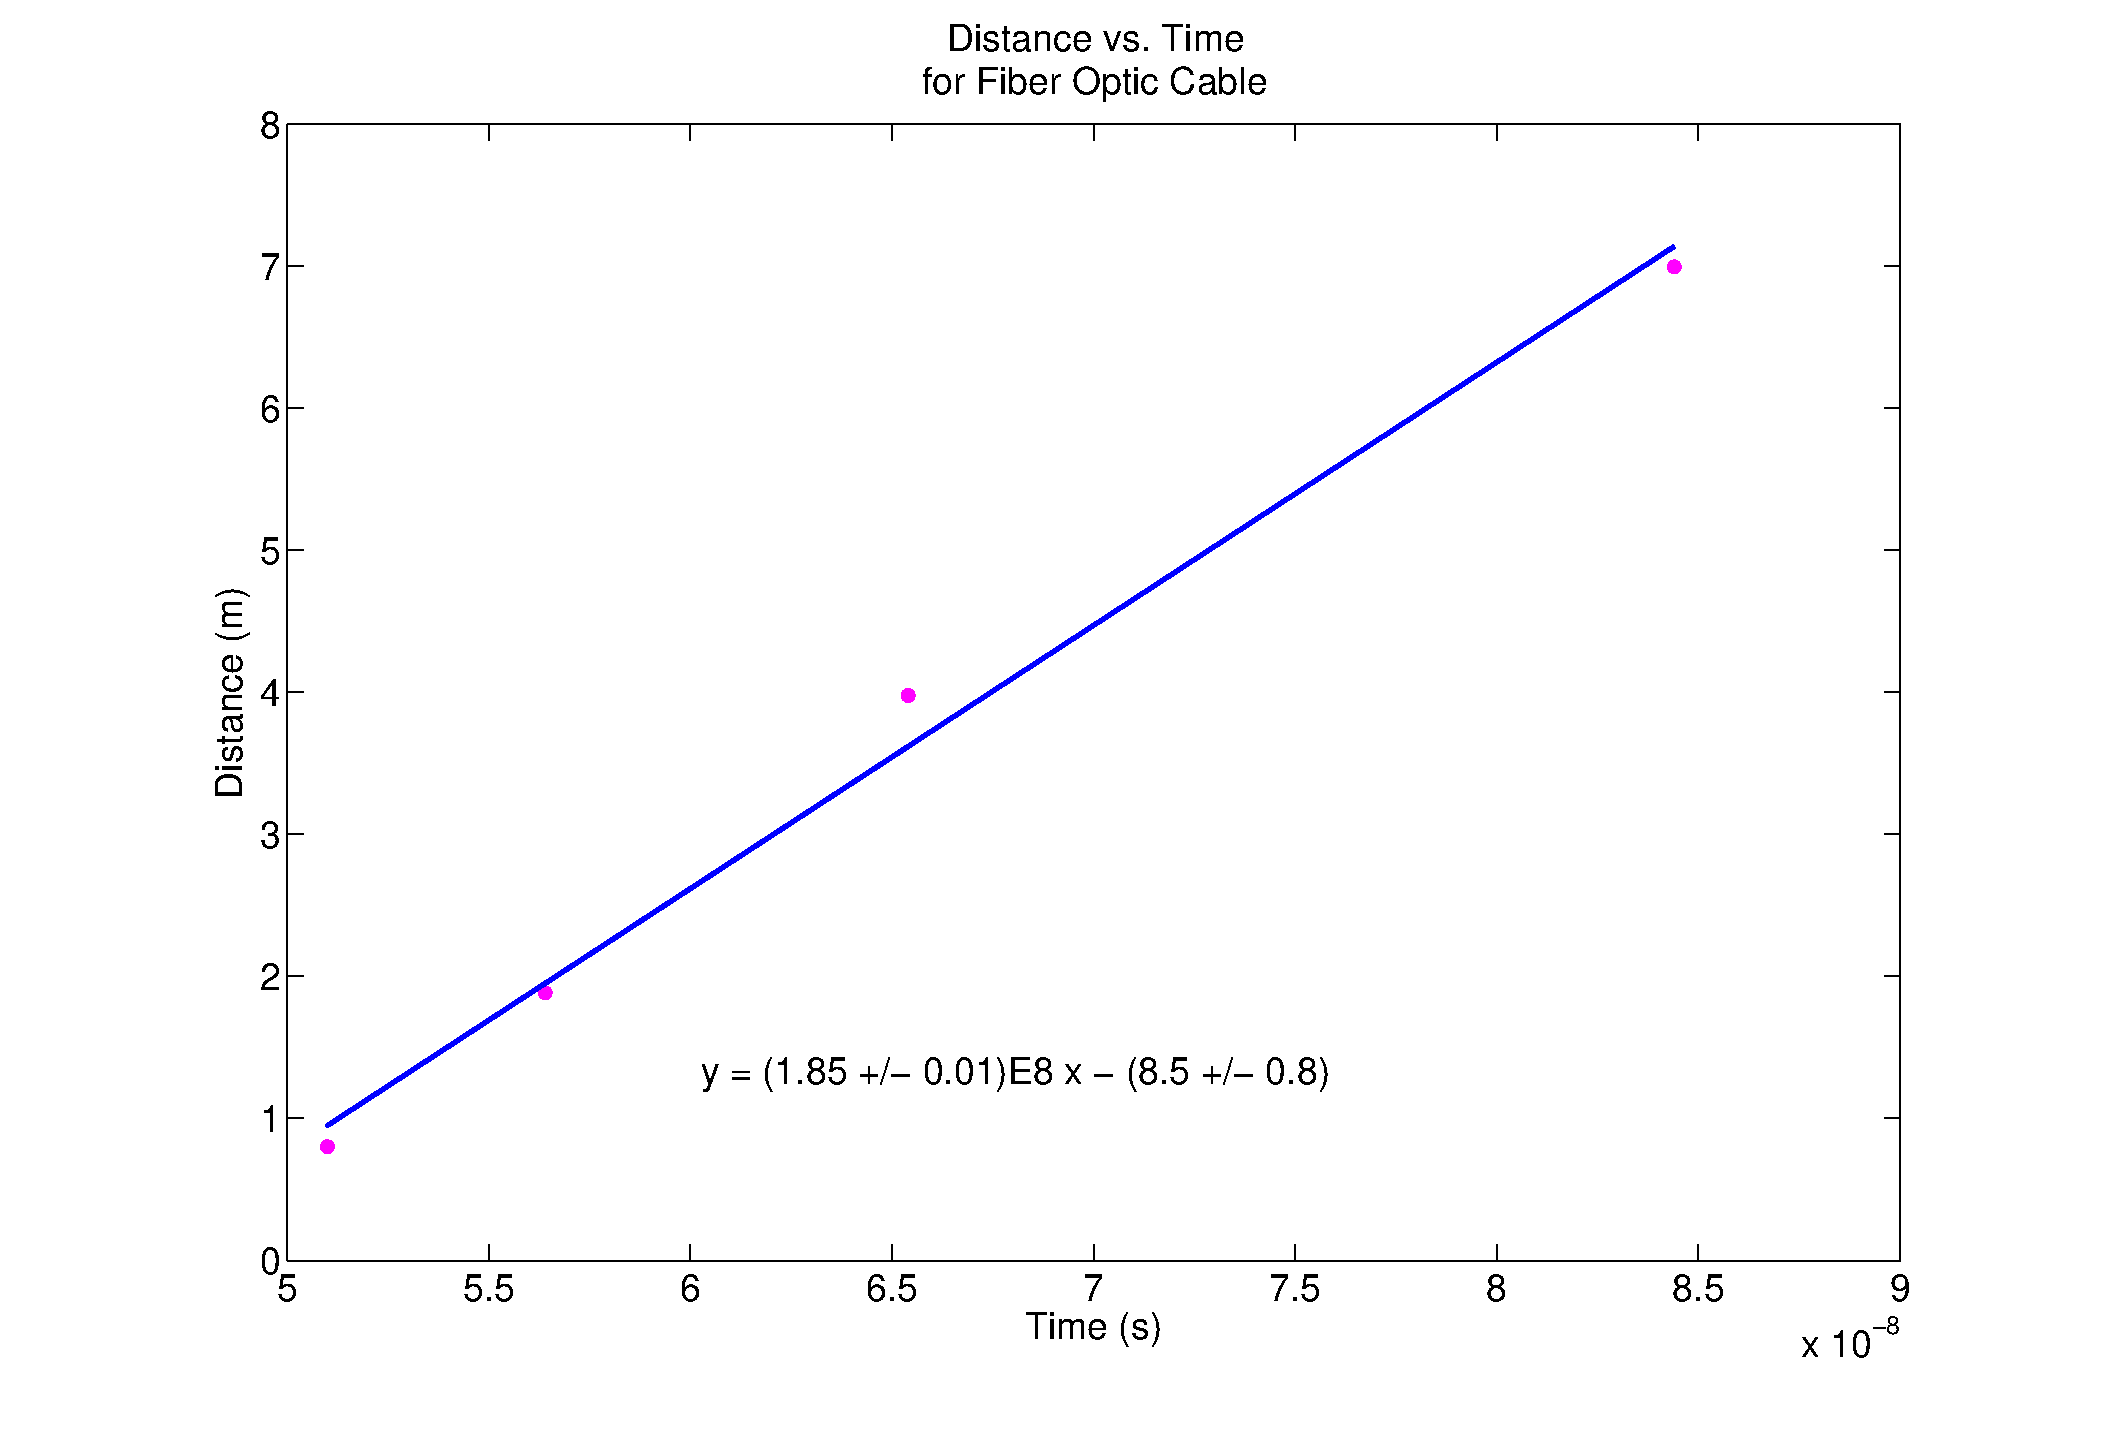
\includegraphics[totalheight=0.6\textwidth]{figs/fiber_final}
  \caption{Determining the speed of light in optical fiber}
  \label{fiber}
\end{figure}
\subsection{Light speed in a coaxial cable}
We propagated electromagnetic waves in a RG-6/U coaxial cable terminated by a resistor box. Depending on the resistance of the box we observed the signal at the end of the cable be: reflected, inverted and absorbed. We measured the speed of an electromagnetic wave in the cable, $c^{\mathrm{cable}} = 2.32 \times 10^{8}$. We determined the velocity factor = 0.79, which agrees with the accepted velocity factor for a RG-6/U coaxial cable = 0.82 \cite{cable}.

\begin{thebibliography}{99}

\bibitem{manual} Physics Dept., ``The Speed of Light'', Quantum Lab,
  California Polytechnic University, (2013).

\bibitem{wiki} ``Optical fiber.'' Wikipedia: The Free Encyclopedia. Wikimedia Foundation, Inc., 05 December 2013. Web.

\bibitem{cable} C. R. Parashare, and R. F. Bradley, ``75 $\Omega$ Transmission System'', National Radio Astronomy Observatory Technology Center, Virginia, 2006.

\end{thebibliography}

\end{document}
